  \item For the spherical surface $x^2 + y^2 + z^2 = 1$, the unit outward normal vector at the point $\left(\tfrac{1}{\sqrt{2}}, \tfrac{1}{\sqrt{2}}, 0\right)$ is given by
  \hfill{(PI 2012)}
  \begin{multicols}{4}
  \begin{enumerate}
    \item $\tfrac{1}{\sqrt{2}} \, \hat{i} + \tfrac{1}{\sqrt{2}} \, \hat{j}$
    \item $\tfrac{1}{\sqrt{2}} \, \hat{i} - \tfrac{1}{\sqrt{2}} \, \hat{j}$
    \item $\hat{k}$
    \item $\tfrac{1}{\sqrt{3}} \, \hat{i} + \tfrac{1}{\sqrt{3}} \, \hat{j} + \tfrac{1}{\sqrt{3}} \, \hat{k}$
  \end{enumerate}
\end{multicols}
  \item The area enclosed between the straight line $y=x$ and the parabola $y=x^2$ in the $xy$-plane is

  \hfill{(PI 2012)}
  \begin{multicols}{4}
  \begin{enumerate}
    \item 1/6
    \item 1/4
    \item 1/3
    \item 1/2
  \end{enumerate}
\end{multicols}
\item  The system of algebraic equations given below has
\hfill{(PI 2012)}
  \begin{align*}
x + 2y + z &= 4 \\
2x + y + 2z &= 5 \\
x - y + z &= 1
\end{align*}
\begin{enumerate}
\item A unique solution of $x=1, y=1$ and $z=1$.
\item Only two solutions of $(x=1, y=1, z=1)$ and $(x=2, y=1, z=0)$.
\item Infinite number of solutions.
\item No feasible solution.
\end{enumerate}
%
\item  For the matrix $A=\myvec{5 & 3 \\ 1 & 3}$, ONE of the normalized eigenvectors is given as
\hfill{(PI 2012)}
  \begin{multicols}{4}
\begin{enumerate}
\item $\myvec{\tfrac{1}{2} \\ \tfrac{\sqrt{3}}{2}}$
\item $\myvec{\tfrac{1}{\sqrt{2}} \\ -\tfrac{1}{\sqrt{2}}}$
\item $\myvec{\tfrac{3}{\sqrt{10}} \\ -\tfrac{1}{\sqrt{10}}}$
\item $\myvec{\tfrac{1}{\sqrt{5}} \\ \tfrac{2}{\sqrt{5}}}$
\end{enumerate}
\end{multicols}
\item A thin square plate $ABCD$ with side of unit length is kept in the $X$-$Y$ plane as shown in the figure. The plate is first rotated by $30^\circ$ in the anti-clockwise direction about the $Z$-axis with $A$ fixed at the origin. The plate is then rotated by $90^\circ$ in the anti-clockwise direction about the $X$-axis with $A$ fixed at the origin. The final co-ordinates of $C$ are
\hfill{(PI 2012)}
\begin{figure}[h!]
\centering
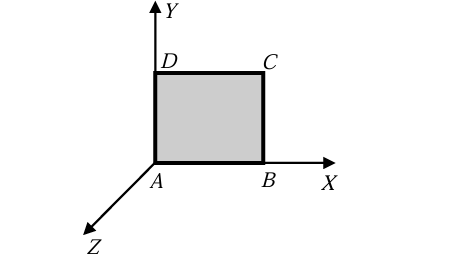
\includegraphics[width=0.35\textwidth]{GATE/2012/PI/figs/39-GATE-PI-2012.png}
\caption{}
\label{q39}
\end{figure}
  \begin{multicols}{2}
\begin{enumerate}
\item (1.366, 0.366, 0.0)
\item (0.0, 1.366, 0.366)
\item (1.366, 0.0, 0.366)
\item (0.366, 0.0, 1.366)
\end{enumerate}
\end{multicols}

